\documentclass[aspectratio=169, handout]{beamer}

\usetheme{Goettingen}

\usepackage{tabularx}
\usepackage{amsmath}
\DeclareMathOperator*{\argmax}{arg\,max}

\title{Text Classification with Python}
\author{Majid Hajiheidari}

\begin{document}
	\frame{\titlepage}
	\section{Introduction: Divar Dataset}
	\frame{
		\frametitle{Divar Posts Dataset}
		\begin{columns}
			\begin{column}{.5\textwidth}
				\begin{itemize}
					\item<2-> Released for DataDays 2019
					\item<3-> One million posts
				\end{itemize}
			\end{column}
			\begin{column}{.5\textwidth}
				%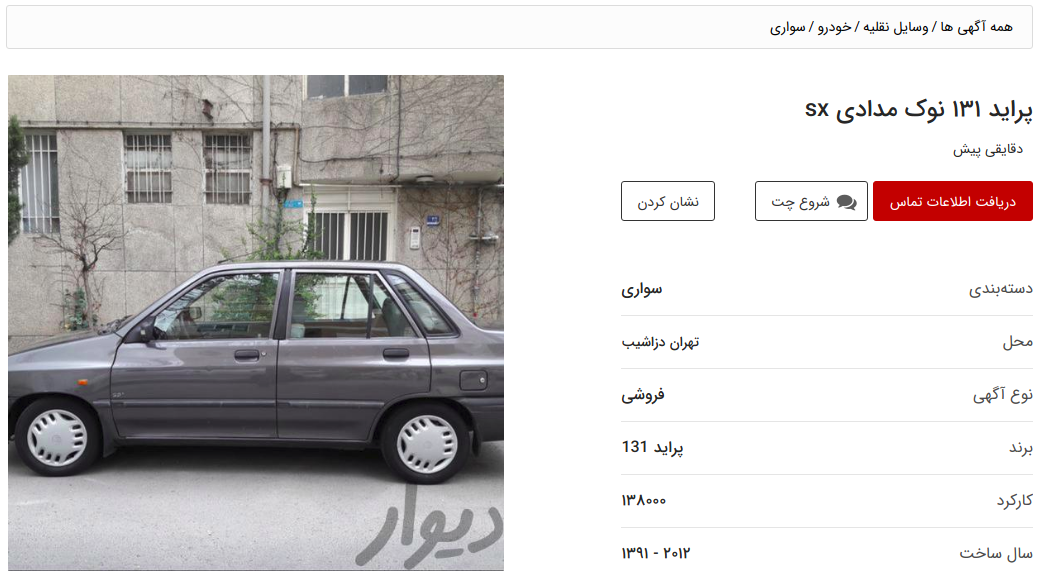
\includegraphics[height=\linewidth]{post1.png}
				
\includegraphics[width=\linewidth]{post2.png}
				
\includegraphics[width=\linewidth]{post3.png}
			\end{column}
		\end{columns}		
	}
	\frame{
		\frametitle{Columns}
		\begin{itemize}
			\item id
			\item archive\_by\_user
			\item published\_at
			\item  \textbf <2> {cat1}
			\item  \textbf <2> {cat2}
			\item  \textbf <2> {cat3}
			\item city
			\item  \textbf <2> {title}
			\item  \textbf <2> {desc}
			\item price
			\item image\_count
			\item platform
			\item mileage
			\item brand
			\item year
			\item type
		\end{itemize}
	}
%	\frame{
%		\frametitle{Title, Description, and Category}
%		\begin{tabular}{l|l|l|l|l}
%			\textbf{Title} & \textbf{Description} & \textbf{Cat1} & \textbf{Cat2} & \textbf{Cat3}\\
%			\hline
%			1&2&3&4&5
%		\end{tabular}
%		\\Some text
%	}
	\section{The Problem: Categorization}
		\frame{
			\frametitle{The Problem: Categorization}
			\begin{itemize}
				\item <2-> We need to categorize posts based on other posts features;
				\item <3-> We only use text features(title \& description)!
			\end{itemize}
		}
		\subsection{Features}
			\frame{
				\frametitle{Temp Frame}
				This slide is temp.
			}
		\subsection{No. of Classes}
			\frame{
				\frametitle{Temp Frame}
				This slide is temp.
			}
	\section{First approach: Naive Bayes}
		\frame{
			\frametitle{First Approach: Naive Bayes Classifier}
			\begin{columns}
				\begin{column}{.5\textwidth}
					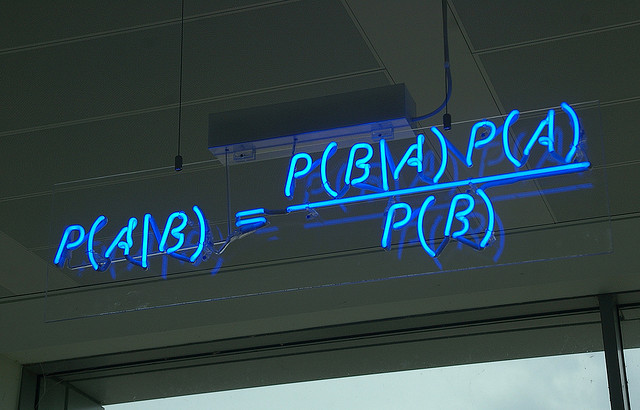
\includegraphics[width=\linewidth]{bayes_formula.jpg}
					\begin{center}
						Photo by \href{https://www.flickr.com/photos/mattbuck007/3676624894}{Matt Buck}
					\end{center}
				\end{column}
				\begin{column}{.5\textwidth}
					\begin{center}
						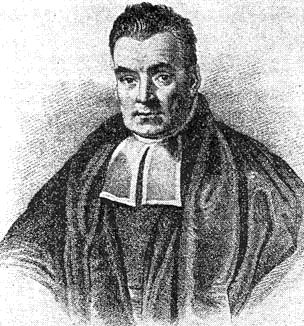
\includegraphics[width=.8\linewidth]{Thomas_Bayes.png}
					\end{center}
				\end{column}
			\end{columns}
		}
		\subsection{Count Vectorizer}
			\frame{
				\frametitle{Vectorizing the Text: Count Vectorizer}
				An example: We want to vectorize these 4 setences\footnote{Example from \href{https://github.com/rahulvasaikar/Bag-of-words}{Rahul Vasaikar}}:\\
				\begin{enumerate}
					\item Hello, how are you!
					\item Win money, win from home.
					\item Call me now
					\item Hello, Call you tomorrow?
				\end{enumerate}
			}
			\frame{
				\frametitle{Vectorizing the Text: Count Vectorizer}
				\begin{enumerate}
					\item We first build a vocabulary:\\
					\begin{math}
					vocabulary = \left\{are, call, from, hello, home, how, me, money, now, tomorrow, win, you\right\}
					\end{math}
					\item Then, we vectorize each sentence based on the occurness of each word:
					\footnotesize\begin{tabular}{l|llllllllllll}
						& are & call & from & hello & home & how & me & money & now & tom... & win & you \\\hline
						1       & 1   & 0    & 0    & 1     & 0    & 1   & 0  & 0     & 0   & 0        & 0   & 1   \\
						2 & 0   & 0    & 1    & 0     & 1    & 0   & 0  & 1     & 0   & 0        & 2   & 0   \\
						3               & 0   & 1    & 0    & 0     & 0    & 0   & 1  & 0     & 1   & 0        & 0   & 0   \\
						4 & 0   & 1    & 0    & 1     & 0    & 0   & 0  & 0     & 0   & 1        & 0   & 1  
					\end{tabular}
				\end{enumerate}
			}
			\frame{
				\frametitle{Vectorizing the Text: Count Vectorizer}
				N pair of samples
			}
		\subsection{Bayes Classifier}
			\frame{
				\frametitle{Bayes Classifier: Naive One!}
				It is possible to show that accuracy is minimized, on average, by a
				very simple classifier that assigns each observation to the most likely class,
				given its predictor values. In other words, we should simply assign a test
				observation with predictor vector $x_0$ to the class j for which\\
				\begin{center}
					\begin{math}
						P\left(Y=j\ \middle|\ \bold{X}=\bold{x}\right)
					\end{math}
				\end{center}
				is largest.
			}
			\frame{
				\frametitle{Bayes Classifier: Naive One!}
				We make two assumptions:
				\begin{enumerate}
					\item $X_1, X_2, \ldots, and\ X_m$ are independent from each other;
					\item $X_1, X_2, \ldots, X_m\mid Y \thicksim MN(\cdot, p_1, p_2, \ldots, p_m)$
				\end{enumerate}
				{\small\begin{align*}
					P(Y=j\mid\bold{X}=(x_1, x_2, \ldots, x_m))
					 &= \frac{P(\bold{X}=(x_1, x_2, \ldots, x_m)\mid Y=j)\cdot P(Y=j)}{P(\bold{X}=\bold{x})}\\
					 &= \frac{P(X_1=x_1\mid Y=j)\cdot\ldots\cdot P(X_m=x_m\mid Y=j)\cdot P(Y=j)}{P(\bold{X}=\bold{x})}.
				\end{align*}}
				\begin{align*}
					\hat{y} = \argmax_{j\in classes} \frac{P(X_1=x_1\mid Y=j)\cdot\ldots\cdot P(X_m=x_m\mid Y=j)\cdot P(Y=j)}{P(\bold{X}=\bold{x})}\\
					=\argmax_{j\in classes} P(X_1=x_1\mid Y=j)\cdot\ldots\cdot P(X_m=x_m\mid Y=j)\cdot P(Y=j).
				\end{align*}
			}
			\frame{
				\frametitle{Bayes Classifier: Naive One!}
				Let's dive into code!
			}
		\subsection{Hyperparameters}
			\frame{
				\frametitle{Hyperparameters}
				Two important hyperparameters:
				\begin{enumerate}
					\item Size of the vocabulary;
					\item Laplace/ Lidstone smoothing parameter($\alpha$).
				\end{enumerate}
			}
			\frame{
				\frametitle{Size of Vocabulary}
				\begin{center}
					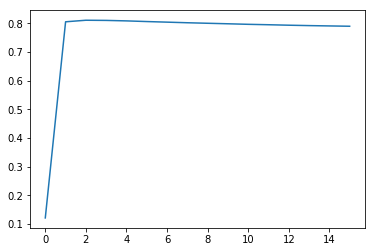
\includegraphics[width=.6\linewidth]{plot1.png}\\
					It is convex!
					(to be completed)
				\end{center}
			}
			\frame{
				\frametitle{Laplace/ Lidstone Smoothing Parameter($\alpha$)}
				\begin{center}
					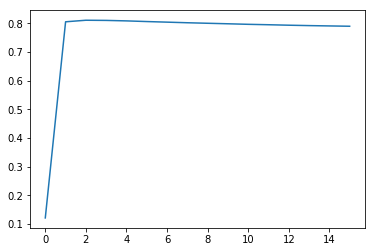
\includegraphics[width=.6\linewidth]{plot1.png}\\
					It is convex!
					(to be completed)
				\end{center}
			}
			\frame{
				\frametitle{Grid Search}
			}
	\section{Second approach: CNN}
		\subsection{Sequence of vectors}
			\frame{
				\frametitle{Temp Frame}
				This slide is temp.
			}
		\subsection{How We Embed}
			\frame{
				\frametitle{Temp Frame}
				This slide is temp.
			}
		\subsection{Patterns with CNN}
			\frame{
				\frametitle{Temp Frame}
				This slide is temp.
			}
		\subsection{Dense Classifier}
			\frame{
				\frametitle{Temp Frame}
				This slide is temp.
			}
	\section{The End}
	\frame{
		\frametitle{Thanks for your attention!}
		Codes in slides (in my GitHub):(github link)\\
		Divar posts dataset:(divar link)\\
		Any questions?\\
		
	}
\end{document}